\documentclass[fontsize=12pt,
% headinclude,
 twoside=false, parskip=half+, numbers=noenddot, plainheadsepline, toc=listof
 %, toc=bibliography
 ]{scrreprt}
% PDF-Kompression
\pdfminorversion=5
\pdfobjcompresslevel=1
% Allgemeines
\usepackage[automark]{scrpage2} % Kopf- und Fußzeilen
\usepackage{amsmath,marvosym} % Mathesachen
\usepackage[T1]{fontenc} % Ligaturen, richtige Umlaute im PDF
\usepackage[utf8]{inputenc}% UTF8-Kodierung für Umlaute usw

\usepackage{geometry}
\geometry{a4paper,left=50mm,right=30mm, top=1cm, bottom=2cm}
% Schriften
\usepackage{mathpazo} % Palatino für Mathemodus
%\usepackage{mathpazo,tgpagella} % auch sehr schöne Schriften
\usepackage{setspace} % Zeilenabstand
\onehalfspacing % 1,5 Zeilen
% Schriften-Größen
\setkomafont{chapter}{\Large\rmfamily} % Überschrift der Ebene
\setkomafont{section}{\large\rmfamily}
\setkomafont{subsection}{\rmfamily}
\setkomafont{subsubsection}{\rmfamily}
\setkomafont{chapterentry}{\large\rmfamily} % Überschrift der Ebene in Inhaltsverzeichnis
\setkomafont{descriptionlabel}{\bfseries\rmfamily} % für description Umgebungen
\setkomafont{captionlabel}{\small\bfseries}
\setkomafont{caption}{\small}
% Sprache: Deutsch
\usepackage[ngerman]{babel} % Silbentrennung
% PDF
\usepackage[ngerman]{hyperref}
\usepackage[final]{microtype} % mikrotypographische Optimierungen
\usepackage{url}
\usepackage{pdflscape} % einzelne Seiten drehen können
% Tabellen
\usepackage{multirow} % Tabellen-Zellen über mehrere Zeilen
\usepackage{multicol} % mehre Spalten auf eine Seite
\usepackage{tabularx} % Für Tabellen mit vorgegeben Größen
\usepackage{longtable} % Tabellen über mehrere Seiten
\usepackage{array}
%  Bibliographie
%\usepackage{bibgerm} % Umlaute in BibTeX
% Tabellen
\usepackage{float}
\usepackage{wrapfig}
% Bilder
\usepackage{graphicx} % Bilder
\usepackage{color} % Farben
\usepackage{colortbl}%Hintergrundfarben für Tabellen	
% Define user colors using the RGB model
\definecolor{dunkelgrau}{rgb}{0.8,0.8,0.8}
\definecolor{hellgrau}{rgb}{0.95,0.95,0.95}
\definecolor{red}{rgb}{1.0,0.5,0.5}
\graphicspath{{images/}}
\DeclareGraphicsExtensions{.pdf,.png,.jpg} % bevorzuge pdf-Dateien
\usepackage{subfigure} % mehrere Abbildungen nebeneinander/übereinander
\newcommand{\subfigureautorefname}{\figurename} % um \autoref auch für subfigures benutzen
\usepackage[all]{hypcap} % Beim Klicken auf Links zum Bild und nicht zu Caption gehen
% Bildunterschrift
\setcapindent{0em} % kein Einrücken der Caption von Figures und Tabellen
\setcapwidth[c]{0.9\textwidth}
\setlength{\abovecaptionskip}{0.2cm} % Abstand der zwischen Bild- und Bildunterschrift
% Quellcode
\usepackage{listings} % für Formatierung in Quelltexten
\definecolor{grau}{gray}{0.25}
\definecolor{lightgray}{rgb}{.9,.9,.9}
\definecolor{darkgray}{rgb}{.4,.4,.4}
\definecolor{purple}{rgb}{0.65, 0.12, 0.82}

\lstdefinelanguage{JavaScript}{
  keywords={typeof, new, true, false, catch, function, return, null, catch, switch, var, if, in, while, do, else, case, break},
  keywordstyle=\color{blue}\bfseries,
  ndkeywords={class, export, boolean, throw, implements, import, this},
  ndkeywordstyle=\color{darkgray}\bfseries,
  identifierstyle=\color{black},
  sensitive=false,
  comment=[l]{//},
  morecomment=[s]{/*}{*/},
  commentstyle=\color{purple}\ttfamily,
  stringstyle=\color{red}\ttfamily,
  morestring=[b]',
  morestring=[b]"
}
\lstset{
   language=JavaScript,
   backgroundcolor=\color{lightgray},
   extendedchars=true,
   basicstyle=\scriptsize\ttfamily,
   showstringspaces=false,
   showspaces=false,
   %numbers=right,
   numberstyle=\scriptsize\ttfamily,
   numbersep=9pt,
   tabsize=2,
   breaklines=true,
   showtabs=false,
   captionpos=b
}
%\lstset{
%	extendedchars=true,
%	%basicstyle=\small\ttfamily,
%	language=java,
%	basicstyle=\footnotesize\ttfamily,
%	tabsize=2,
%	keywordstyle=\textbf,
%	commentstyle=\color{grau},
%	stringstyle=\textit,
%	numbers=left,
%	numberstyle=\small,
%	% für schönen Zeilenumbruch
%	breakautoindent  = true,
%	breakindent      = 2em,
%	breaklines       = true,
%	postbreak        = ,
%	prebreak         = \raisebox{-.8ex}[0ex][0ex]{\Righttorque},
%}
% linksbündige Fußboten
\deffootnote{1.5em}{1em}{\makebox[1.5em][l]{\thefootnotemark}}

%\typearea{14} % typearea am Schluss berechnen lassen, damit die Einstellungen oben berücksichtigt werden
% für autoref von Gleichungen in itemize-Umgebungen
\makeatletter
\newcommand{\saved@equation}{}
\let\saved@equation\equation
\def\equation{\@hyper@itemfalse\saved@equation}
\makeatother 


 % Importiere die Einstellungen aus der Präambel
% hier beginnt der eigentliche Inhalt
\begin{document}
\pagenumbering{Roman} % große Römische Seitenummerierung
\pagestyle{empty}

% Titelseite
\clearscrheadings\clearscrplain

\begin{center}
\begin{Huge}
Institut für Mathematik und Informatik\\
\vspace{3mm}
\end{Huge}{\Large Fernuniversiät Hagen}\\

\vspace{20mm}
\begin{Large}
Vergleichende Implementierung und Evaluierung einer ereignisgesteuerten, nicht
blockierenden I/O Lösung für eine datenintensive Real-Time Webanwendung in Javascript
und Dart\\
\end{Large}
\vspace{8mm}
Bachelorarbeit\\
\vspace{0.4cm}
\vspace{2 cm}
Barbara Drüke \\
Matrikel-Nummer 7397860\\
\vspace{5cm}
\begin{tabular}{ll}
{\bf Betreuer} & Dr. Jörg Brunsmann\\
{\bf Erstprüfer}&Prof. Hemmje\\
{\bf Zweitprüfer}&Dr. Jörg Brunsmann\\
\end{tabular}

\end{center}
\clearpage


\pagestyle{useheadings} % normale Kopf- und Fußzeilen für den Rest

\tableofcontents
\listoffigures
\listoftables





% richtiger Inhalt
%---------------------------------------------------------------------------------------------------------------------------------------------
\chapter{Einleitung}
\pagenumbering{arabic} % ab jetzt die normale arabische Nummerierung

Die Vesseltracker.com GmbH ist ein Schiffsmonitoring und -reporting-Dienstleister. Der kostenpflichtige Dienst stellt den Kunden umfangreiche Informationen zu Schiffen weltweit zur Verfügung. Dabei handelt es sich einerseits um Schiffs-Stammdaten und andererseits um Schiffs-Postionsdaten. Die Positionsdaten sind AIS (Automatic Identification System) -Daten, wie sie von allen Schiffen über Funk regelmäßig zu senden sind.

\begin{wrapfigure}{r}{0.6\textwidth}
  \begin{center}
    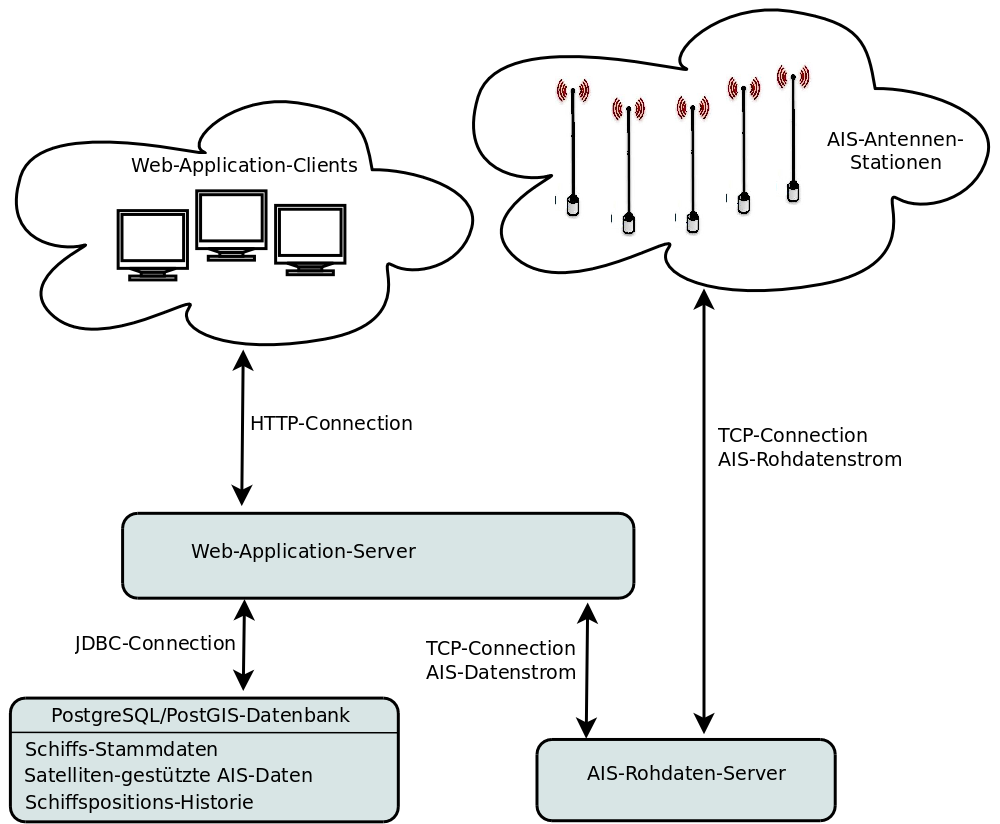
\includegraphics[width=0.58\textwidth]{images/Exposee_graphik_Webapp}
  \end{center}
  \caption{Vesseltracker\_Webapplikation}
\end{wrapfigure}

Vesseltracker.com unterhält ein Netzwerk von ca. 800 terrestrischen AIS-Antennen, mit denen küstennahe AIS-Meldungen empfangen und via Internet an einen zentralen Rohdatenserver geschickt werden. Der Rohdatenserver verarbeitet die Meldungen und gibt sie umgewandelt und gefiltert an die Anwendungen des Unternehmens weiter.
Zusätzlich erhält das Unternehmen AIS-Daten via Satellit über einen Kooperationspartner. Damit werden die küstenfernen Meeresgebiete und Gegenden, in denen Vesseltracker.com keine AIS-Antenne betreibt, abgedeckt.
Die Kernanwendung des Unternehmens ist eine Webanwendung, die die terrestrischen AIS-Daten in einer Geodatenbank speichert und sie mit den Schiffs-Stammdaten und Satelliten-AIS-Daten in Beziehung setzt.

Für eine geographische Visualisierung der Schiffspositionen existiert das sogenannte 'Cockpit', wo die Schiffe als Icons auf Openstreetmap-Karten dargestellt werden. Diese Karte zeigt jeweils alle Schiffe an, die sich in dem frei wählbaren Kartenausschnitt zu der Zeit befinden. Aktualisiert werden die Positioninformationen jeweils bei Änderung des betrachteten Bereichs  oder einmal pro Minute. Detailinformationen erhält der Nutzer durch ein Click-Popup über das Icon des Schiffes. Darüber kann er sich auch die gefahrene Route der letzten 24 h anzeigen lassen.


\begin{figure}[H]
  \centering
  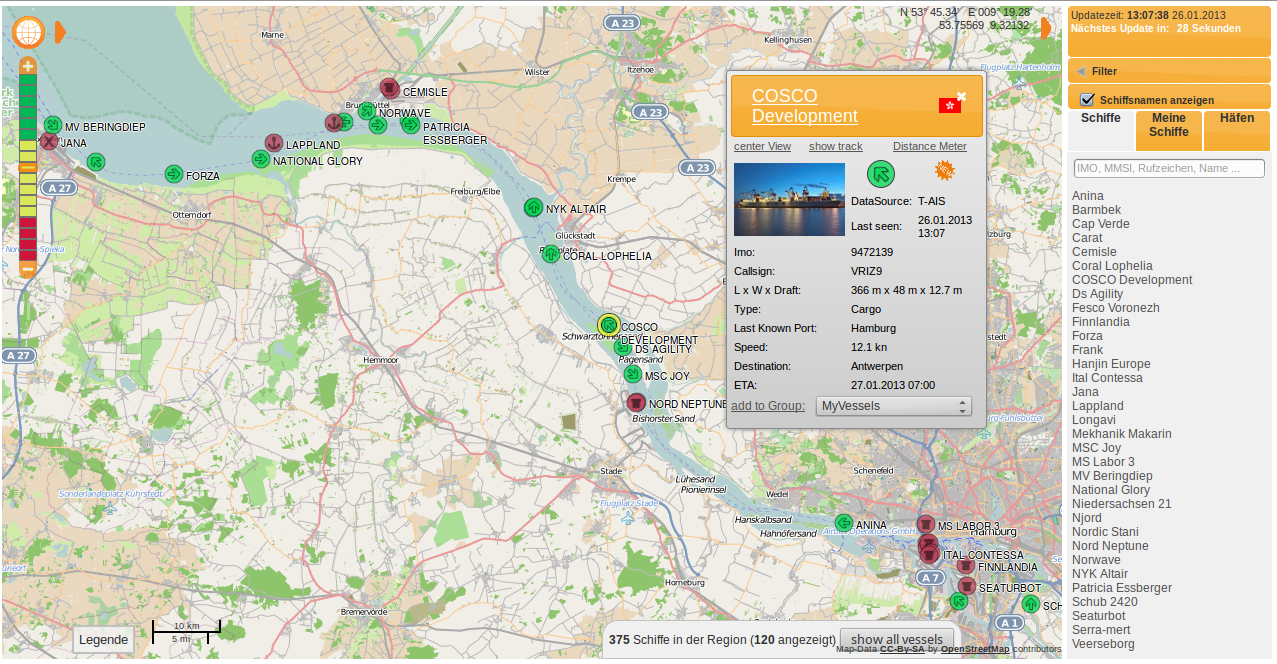
\includegraphics[width=6in]{images/Cockpit_Elbe}
  \caption[Cockpit\_Elbe]{Cockpit\_Elbe}
\end{figure}

\section{Motivation für diese Arbeit}\label{s.Motivation für diese Arbeit}

Weil in letzter Zeit real-time-Anwendungen zunehmend an Bedeutung gewinnen und ihre Verbreitung durch den Fortschritt der verfügbaren Webtechnologien auf breiter Basis unterstützt wird, entstand die Idee, alternativ zur Cockpit-Anwendung eine real-time-Darstellung der Schiffsbewegungen als Browseranwendung anzubieten. Aufgrund der hohen Aktualisierungsrate der empfangenen AIS-Daten entstünde damit eine dynamische Präsentation von Schiffsbewegungen, die das tatsächliche Geschehen auf dem Wasser nahezu sekundengenau wiederspiegelt. So wäre es dem Kunden möglich, Situationen wie Anlegen, Festmachen, Ablegen und Schleusendurchfahrten oder Manöver wie Schleppen, Lotsen oder Betanken 'live' mitzuverfolgen.

\section{Aufbau der Arbeit}\label{s.Aufbau der Arbeit}
Im Kapitel 2 werden mögliche Anwendungs-Szenarien genauer beleuchtet und die funktionalen und nicht funktionalen Anforderungen an die geplante Anwendung herausgestellt. Anschließend wird die Systemarchitektur der geplanten Anwendung grob entworfen.
Kapitel 3.1 gibt eine kurze Einführung in die Websocket-Technologie, Kapitel 3.2 in die Programmiersprache Google Dart.
Kapitel 4 begründet die getroffene Auswahl an Websockets und schildert die Vorgehensweise der Implementierung, wobei Teile der Implementierung vorgestellt werden.
Die ausgearbeiteten Implementierungen werden dann in Kapitel 5 nach verschiedenen Aspekten verglichen und die Ergebnisse in Kapitel 6 zusammengefasst.

%---------------------------------------------------------------------------------------------------------------------------------------------
\chapter{Realtime-Schiffsverfolgung per AIS-Daten-Strom}\label{c.Realtime-Schiffsverfolgung per AIS-Daten-Strom}

\section{ Anwendungsfälle}\label{s.Anwendungsfälle}

Ein Repräsentant des Unternehmens vesseltracker.com nutzt die Realime-Anwendung auf einer Schifffahrtsmesse, um potentiellen Kunden die hohe Qualität der von Vesseltracker angebotenen AIS-Daten zu präsentieren. Dabei ist es wichtig, dass die Anwendung gesendete AIS-Signale im Schnitt in weniger als einer Sekunde auf dem Monitor als Position oder Positionsänderung darstellen kann. Damit kann vesseltracker.com die Überlegenheit der eigenen Daten bezüglich Genauigkeit und Aktualität gegenüber denen anderer Anbieter herausstellen.

Hafendienstleister wie Schlepper, Lotsen oder Festmacher verschaffen sich über einen Monitor einen Überblick über die Arbeitsvorgänge in ihrem jeweiligen Heimathafen. Sie kontrollieren die eigenen Aufträge oder auch die der Mitbewerber.
Die Anwendung läuft hierbei eher statisch, das heißt Zoomstufe und Kartenausschnitt ändern sich nur selten. Es ist also notwendig, dass die Anwendung unabhängig von Aktionen des Nutzers sich laufend oder regelmäßig aktualisiert.
%Welche Schlepper schleppen welches Schiff?
%Wo geht der Lotse an Bord, wo verlässt er das Schiff?
%Welcher Tanker betankt welchen Frachter?

Reedereien beobachten das Einlaufen, Festmachen, Ablegen ihrer Schiffe in entfernten Häfen, wo es keine Unternehmensniederlassung gibt. Zum Beispiel kontrollieren sie, an welchem Liegeplatz ein Frachtschiff wie lang festmacht?
Dazu ist es zum einen notwendig, jederzeit auf eine geringe Zoomstufe heraus- und auf einen anderen Hafen wieder hineinzoomen zu können. Zum anderen soll die Anwendung Schnittstellen bieten, wie Informationen aus dem vesseltracker.com Datenpool (in diesem Fall Liegeplatzinformationen) der Anwendung hinzugefügt werden können.






Welche Hafendienstleister (Schlepper, Lotsen, Festmacher) sind an dem Manöver beteiligt?
Nutzer der Passagierschifffahrt setzen sich in Kenntnis über die Position von Fähren.
Freunde der Schifffahrt / Schiffsfotografen beobachten die Routen von Schiffen von besonderem Interesse.
Die Wasserschutzpolizei hat ein zusätzliches Werkzeug zur Kontrolle der Geschehnisse auf dem Wasser.
Die Anwendungsfälle verdeutlichen noch einmal, dass der zusätzliche Nutzen der Realtimeanwendung gegenüber der Cockpitanwendung nicht in erster Linie im Informationsgehalt liegt. Die Daten im Cockpit sind ja ebenfalls im Minutenbereich aktuell. Der Vorteil liegt vielmehr in der Lebendigkeit der Darstellung. Bewegte Darstellungen binden stärker und für einen längeren Zeitraum die Aufmerksamkeit des Betrachters.

\section{Beschreibung der Anforderungen}\label{s.Beschreibung der Anforderungen}

Die funktionalen Anforderungen sind:
\begin{itemize}

\item als Datenquelle sollen ausschließlich die vom Rohdatenserver als JSON-Datenstrom zur Verfügung gestellten AIS-Informationen dienen
\item Schiffe sollen an ihrer aktuellen (realtime) Position auf einer Karte im Browser dargestellt werden
\item Positionsänderungen einzelner Schiffe sollen ad hoc sichtbar gemacht werden
\item die Schiffsbewegungen auf der Karten sollen nicht sprunghaft, sondern fließend erscheinen (Animation der Schiffsbewegungen in dem Zeitraum zwischen zwei Positionsmeldungen)
\item die Karte soll in 16 Zoomstufen die Maßstäbe von 1:2000 bis 1: 200 Mio abdecken
\item Schiffe sollen auf der Karte als Icons dargestellt werden, die den Navigationsstatus und gegebenenfalls den Kurs wiederspiegeln
\item bei hoher Auflösung und ausreichend statischen AIS-Informationen soll ein Schiff als Polygon in die Karte eingezeichnet werden.
\item bei geringer Auflösung ist ein Überblick über die Verteilung der empfangenen Schiffe zu vermitteln
\item Detail-Informationen zu jedem Schiff sollen als Popups über das Icon abrufbar sein
\end{itemize}

Nicht funktionale Anforderungen sind:
\begin{itemize}
\item die von den Antennen empfangenen AIS-Daten sind mit minimaler Verzögerung (< 500 msec) auf der Karte darzustellen
\item die Anwendung sollte ca. 300 Verbindungen gleichzeitig erlauben und skalierbar sein
\item als Clients der Anwendung sollten die gängigsten Browser unterstützt werden (IE, Chrome, Firefox, Safari, Opera) 
\item die Implementierungen werden auf Github als privates repository gehalten
\item als Kartenmaterial sind die von vesseltracker gehosteten OpenstreetMap-Karten zu verwenden
\item verwendete Software-Module sollten frei zugänglich sein (open source) 
\item ein Prototyp der Anwendung soll schnell zur Verfügung stehen. Dieser Prototyp soll Mitarbeitern und Partnern ermöglichen, ihre Anforderungen genauer zu spezifizieren oder sogar neue Anforderungen zu formulieren. 
\end{itemize}

\section{Grobentwurf der Anwendung}\label{s.Grobentwurf der Anwendung}
Die eingehende Schnittstelle der zu erstellenden Anwendung ist die Verbindung zum Rohdatenserver, die als TCP-Verbindung ausgeführt ist und einen JSON-Datenstrom liefert.
Die ausgehende Schnittstelle ist der HTTP-Client (Browser).
\begin{wrapfigure}{r}{0.6\textwidth}
  \begin{center}
    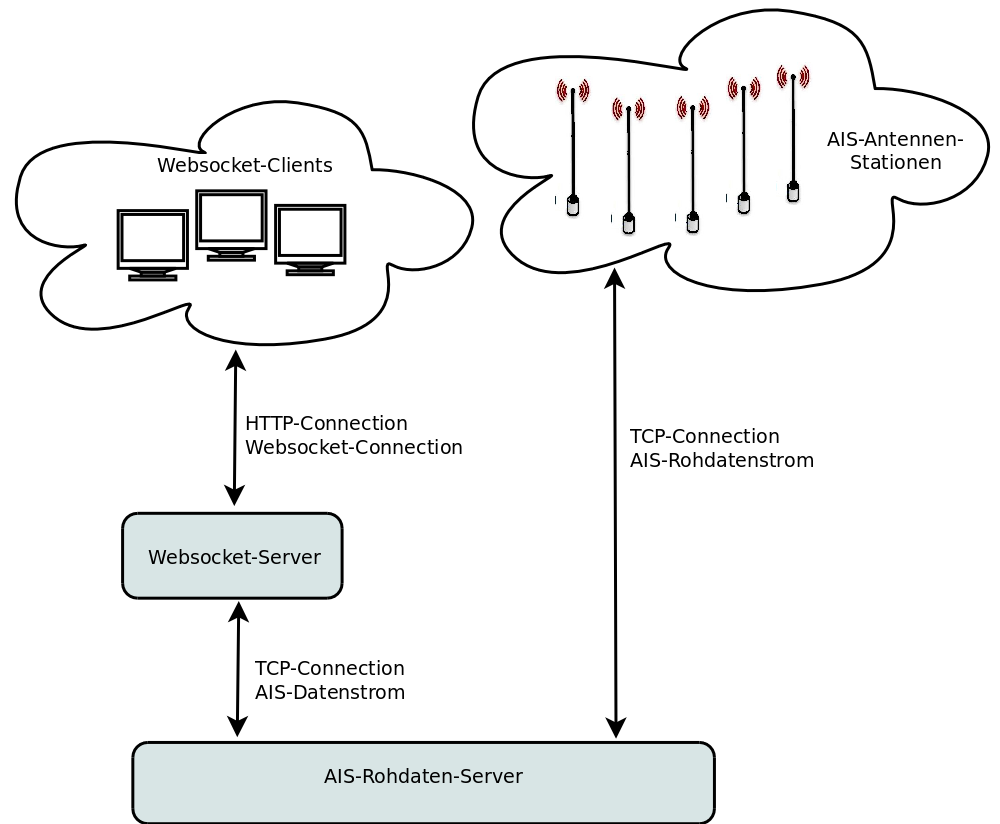
\includegraphics[width=0.58\textwidth]{images/Exposee_graphik_Realtimeapp}
  \end{center}
  \caption{Architektur-Entwurf der Realtime\_Webapplikation}
\end{wrapfigure}

Zu erstellen ist also eine Client-Server-Anwendung, in der der Server zweifaches zu leisten hat, nämlich 
\begin{enumerate}
 \item eine tcp-socket-Verbindung zum Rohdatenserver zu unterhalten und
  \item eine bidirektionale Verbindung zum HTTP-Client zu halten, in der der Client jederzeit Änderungen des betrachteten Kartenausschnittes an den Server senden und der Server jederzeit den Client über relevante, aus dem JSON-Datenstrom ausgelesene, Schiffsbewegungen im betrachteten Kartenausschnitt informieren kann.
\end{enumerate}


%---------------------------------------------------------------------------------------------------------------------------------------------
\chapter{Grundlagen}\label{s.Grundlagen}
\section{Automatisches Informationssystem}\label{s.Automatisches Informationssystem (AIS)}
Das Automatic Identification System (AIS) ist ein UKW-Funksystem im Schiffsverkehr, das seit 2004 für alle Berufsschiffe über 300 BRZ in internationaler Fahrt und seit 2008 auch für solche über 500 BRZ in nationaler Fahrt verpflichtend eingeführt worden ist. Es soll dabei helfen, Kollisionen zwischen Schiffen zu verhüten und die landseitige Überwachung und Lenkung des Schiffsverkehrs zu erleichtern. Außerdem verbessert AIS die Planung an Bord, weil nicht nur Position, Kurs und Geschwindigkeit der umgebenden Schiffe übertragen werden, sondern auch Schiffsdaten (Schiffsname, MMSI-Nummer, Funkrufzeichen, etc.). AIS ist mit UKW-Signalen unabhängig von optischer Sicht und Radarwellenausbreitung.\\
Für die Nutzung von AIS ist ein aktives, technisch funktionsfähiges Gerät an Bord Voraussetzung, das sowohl Daten empfängt als auch Daten sendet. Für Schiffe der Berufsschifffahrt sind Klasse-A-Transceiver an Bord vorgesehen, für nicht ausrüstungspflichtige Schiffe genügen Klasse-B-Transceiver, die mit niedriger VHF-Signalstärke und weniger häufig senden.  \\
Die dynamischen Schiffsdaten (LAT, LON, COG, SOG, UTC) erhält der AIS-Transceiver vom integrierten GPS-Empfänger, bei Klasse A auch von der Navigationsanlage des Schiffes. Die Kursrichtung (Heading =  HDG) kann über eine NMEA-183-Schnittstelle vom Kompass eingespeist werden.

Die AIS-Einheit sendet schiffsspezifische Daten, die von jedem AIS-Empfangsgerät in Reichweite empfangen und ausgewertet werden können:
Statische Schiffsdaten: 
\begin{itemize}
\item IMO-Nummer
\item Schiffsname
\item Rufzeichen
\item MMSI-Nummer
\item Schiffstyp (Frachter, Tanker, Schlepper, Passagierschiff, SAR, Sportboot u. a.)
\item Abmessungen des Schiffes (Abstand der GPS-Antenne von Bug, Heck, Backbord- und Steuerbordseite)
\end{itemize}

Dynamische Schiffsdaten
\begin{itemize}
\item Navigationsstatus (unter Maschine, unter Segeln, vor Anker, festgemacht, manövrierunfähig u. a.)
\item Schiffsposition (LAT, LON, in WGS 84)
\item Zeit der Schiffsposition (nur Sekunden)
\item Kurs über Grund (COG)
\item Geschwindigkeit über Grund (SOG)
\item Vorausrichtung (HDG)
\item Kursänderungsrate (ROT)
\end{itemize}

Reisedaten
\begin{itemize}
\item aktueller maximaler statischer Tiefgang in dm
\item Gefahrgutklasse der Ladung (IMO)
\item Reiseziel (UN/LOCODE)[5]
\item geschätzte Ankunftszeit (ETA)
\item Personen an Bord
\end{itemize}

Der Navigationsstatus und die Reisedaten müssen vom Wachoffizier manuell aktualisiert werden. Gesendet werden die AIS-Signale auf zwei UKW-Seefunkkanälen (Frequenzen 161,975 MHz und 162,025 MHz), wobei die Sendeintervalle abhängig sind von der Klasse, dem Manöverstatus und der Geschwindigkeit.

\begin{table}[!hbt]\vspace{1ex}\centering
\begin{tabular}{|l|l|l|l|}\hline
Klasse &Manöver-Status & Geschwindigkeit &Sendeintervall\\\hline\hline
Class A&geankert/festgemacht&<3kn&3 min\\
Class A&geankert/festgemacht&>3kn&10 sec\\
Class A&in Fahrt&0-14kn&10 sec\\
Class A&in Fahrt, Kursänderung&0-14&3 1/3 sec\\
Class A&in Fahrt&14-23kn&6 sec\\
Class A&in Fahrt, Kursänderung&14-23&2 sec\\
Class A&in Fahrt&>23kn&2 sec\\
Class B&&<2 kn&3 min\\
Class B&&>2 kn&30 sec\\\hline
\end{tabular}
\caption[Intervalle, in denen ein Schiff seine Daten aussendet] {Intervalle, in denen ein Schiff seine Daten aussendet}
\end{table}

Für AIS-Daten sind 22 standardisierte Nachrichtentypen bzw. Telegramme festgelegt:
In dieser Arbeit werden nur Class A Positionsmeldungen betrachtet (Typ 1-3) un.
\begin{table}[!hbt]
\centering
\begin{tabular}{|l|l|}\hline
ID&Nachrichtentyp\\\hline\hline
1& reguläre Positionsmeldung eines Klasse-A-Transceivers\\
4 & Meldung einer Basisstation\\
5& reguläre Meldung von Schiffs- und Reisedaten eines Klasse-A-Transceivers\\
9 & Positionsmeldung eines SAR-Luftfahrzeuges\\
12& sicherheitsbezogene Nachricht - adressiert\\
14& sicherheitsbezogene Nachricht - an alle\\
18& reguläre Positionsmeldung eines Klasse-B-Transceivers\\
21& Positions- und Statusmeldung eines AtoN-Transceivers\\\hline
\end{tabular}
\caption[Die wichtigsten AIS-Telegrammtypen] {Die wichtigsten AIS-Telegrammtypen}
\end{table}

Zur landseitigen AIS-Infrastruktur gehören sogenannte AIS-Basisstationen und AIS-Empfänger. Basisstationen dienen einerseits zur Erfassung des Verkehrs in dem von ihnen abgedecken Seegebiet, andererseits können diese Geräte die Übertragung von AIS-Transceivern an Bord gezielt steuern (z.B. Hochsetzen der Melderate). AIS-Empfänger sind reine AIS-Empfangsgeräte, die keine Daten senden.\\


\section{Bidirektionale Kommunikation über Websockets}\label{s.Bidirektionale Kommunikation über Websockets}

In der Entwicklung der Kommunikationstechnologien im Internet galt lange Zeit das request/response Paradigma, nach dem Anfragen vom Client vom Server beantwortet werden. Dieses Paradigma wird Stück für Stück aufgebrochen duch kontinuierliche Weiterentwicklungen in Richtung einer bidirektionalen Kommunikation zwischen Server und Client.
Mit HTTP Long Polling, HTTP Streaming und Ajax on demand ist es, nachdem der Client eine Verbindung hergestellt hat, für den Server möglich, beim Eintreffen neuer Daten scheinbar selbständig einen Datenaustausch zum Client zu initieren. Dabei handelt es sich eigentlich nur um einen aufgeschobenen response auf einen zuvor gestellten client-Request.
Der Nachteil dieser Technologien liegt darin, dass sie, weil sie http-Nachrichten austauschen, einen großen Überhang an Header-Informationen mitzusenden gezwungen sind, der sich in Summe negativ auf die Verzögerung auswirkt. Damit sind diese Technologien für zeitkritische (realtime) Anwendungen nicht unbedingt geeignet.
Das 2011 eingeführte Websocket-Protokoll dagegen beschreibt eine API, die eine echte bidirektionale Socket-Verbindung zwischen Server und Client ermöglicht, in der beide Seiten jederzeit Daten schicken können. Dieser Socket wird im Anschluss an einen intialen HTTP-handshake aufgebaut, indem Server und Client  einen Upgrade der Verbindung auf das Websocket-Protokoll aushandeln. 


\subsection{HTML5-Websocket API-Spezifikation}
%Um über die Einschränkungen des request/response Musters hinwegzukommen, bei dem Anfragen des Client vom Server beantwortet werden, sind kontinuierlich Fortschritte in Richtung einer bidirektionialen Verbindung zwischen Client und Server gemacht worden.


\subsection{Vorstellung verschiedener  Implementierungen von Websockets}

\subsubsection{Nodejs-Websockets}\label{s.Nodejs-Websockets}

\subsubsection{Dart-Websockets mit Dart:IO}

\section{Google Dart als moderne Programmiersprache für Webanwendungen}\label{s.Google Dart als moderne Programmiersprache für Webanwendungen}


\subsection{Motivation für Dart}

\subsection{Eigenschaften und Besonderheiten der Programmiersprache Dart}\label{s.Eigenschaften und Besonderheiten der Programmiersprache Dart}

\subsection{Dart Tools (DartEditor, dart2js-compiler)}\label{s.Dart Tools (DartEditor, dart2js-compiler)}


\subsection{Einbindung von Javascript-Bibliotheken in Dart mit js-interop}\label{s.Einbindung von Javascript-Bibliotheken in Dart mit js-interop}


%---------------------------------------------------------------------------------------------------------------------------------------------
\chapter{Vorstellung der ausgeführten Implementierungen}\label{s.Implementierungen}

Aus den betrachteten Programmiersprachen (Javascript, Google Dart) und Modulen (node.js, socket.io, dart:io, dart:html) gilt es nun, sinnvolle und vergleichbare Lösungen zu implementieren für die Serveranwendung und die korrespondierenden Clients.

\section{Implementierung des Prototypen in Javascript}
Um der Anforderung nachzukommen, schnell einen funktionierenden Prototypen zu liefern, wird für die erste Implementierung Javascript als Programmiersprache gewählt. Damit ist eine Unterstützung der gängigen Browserclients gewährleistet und eine große Anzahl an Modulen steht zur Verfügung.

Node.js wird als Framework eingebunden, weil node.js 
\begin{itemize}
\item ereignisgesteuerte Verarbeitung unterstützt, was für die Umsetzung der geforderten Funktionalität hilfreich ist,
\item Asynchronizität von I/O-Operationen bietet, womit die Verarbeitungszeit minimal gehalten werden kann,
\item mehrere Websocket-Implementierungen anbietet (socket.io, websocket, ws).
\end{itemize}
Für den Websocket wird das socket.io - package genutzt, weil socket.io neben zahlreichen Konfigurationsmöglichkeiten eine breite Browserunterstützung bietet, indem es mit Browsern, die Websockets nicht unterstützen, eine Verbindung auf Basis  älterer Technologien wie http-Polling aufbaut. Dadurch erhöht sich für diese Clients zwar die Latenzzeit, die Funktionalität ist aber gewährleistet.

Im Folgenden wird die hier beschriebene Implementierung socket.io-Server genannt. Der zugehörige Client (socket.io-Client) wird ebenfalls in Javascript implementiert und bindet die socket.io-Bibliotheken ein.

\subsection{socket.io-Server}
Die Serveranwendung hat im Grunde zwei Aufgaben: erstens eine JSON-over-TCP-Verbindung zum Empfang der Daten vom Rohdatenserver und zweitens einen Websocket-Server zur Verteilung der Daten an die Clients.
Weil Node.js singlethreaded ist (\ref{s.Nodejs-Websockets}) würden beide Aufgaben in einem einzigen Prozess bearbeitet. Um das Potential an Parallelverabeitung eines Dualcore oder Multicore-Servers zu nutzen, ist des daher sinnvoll, mindestens zwei Prozesse zu generieren. Dazu wurde das node.js-Modul child\_process genutzt. Die ausführbare Datei master.js generiert damit zuerst einen Prozess, der den AIS-Client (ais\_client.js) startet und anschließend einen Prozess (worker.js), der einen Websocket -Server zur Verfügung stellt.

Der Datenaustausch zwischen beiden Prozessen funktioniert über zwei nosql-Datenbanken. In einer mongo-Datenbank werden alle vom ais\_client-Prozess empfangen Positions- und Reisedaten  unter der mmsi eines Schiffes gespeichert. Dabei wird die upsert-Option von Mongo genutzt, so dass nicht vorhandene Schiffe eingefügt und vorhande aktualisiert werden.

Der worker-Prozess greift auf die Mongo-Datenbank zu, um für einen vom Client angefragten Kartenausschnitt die entsprechenden Schiffe abzufragen. Dabei wird der in Mongo zur Verfügung stehende Geo-Index auf der Schiffsposition verwendet.

Zur Verteilung der Positionsmeldungen (msgid 1,2 und3)  wird außerdem eine Redis-Datenbank verwendet, die über einen publish/subscribe-Mechanismus verfügt. Über einen Kanal "vesselpos" publiziert der AIS-Client-Prozess die Positionsmeldungen und der worker-Prozess meldet sich am selben Kanal an und wird über jede Positionsmeldung benachrichtigt, die er an seine verbunden Websocket-Clients weiterreichen kann.

\subsection{socket.io-Client}
Das socket.io Paket bietet Features wie die interne Clientverwaltung durch den Websocket.

\section{Vergleichsimplementierung in Google Dart}

Nachdem die Anwendung als Prototyp in Javascript fertiggestellt ist, soll eine vergleichbare Implementierung in Google Dart realisiert werden. Das paket dart:io bietet die entsprechende Unterstützung für HTML5-Websocket-Server und dart:html für HTML5-Websocket-Clients.
Allerdings ergeben sich auf der Serverseite einige schwerwiegende Probleme:
- zum Zeitpunkt der Umsetzung (Dezember 2012) fehlt noch ein Redis-Client in Dart, so dass für die publish/subscribe-Lösung mit Redis [siehe] eine Alternative entwickelt werden müsste, die wiederum die Vergleichbarkeit beider Implementierungen herabsetzt.
- der socket.io-Server nutzt 'JSON over TCP', um die Daten vom Rohdatenserver abzufragen. 'JSON over TCP' ist in Dart (noch) nicht implementiert. Ohne die Schnittstelle zum Rohdatenserver zu verändern ist also keine vergleichbare Lösung in Dart umsetzbar.

Der Vergleich zwischen der Javascript- und der Google Dart-Anwendung ist also zu diesem Zeitpunkt lediglich auf der Clientseite möglich beziehungsweise sinnvoll. 
Websocketverbindungen werden in Dart clientseitig mit dem Paket dart:html unterstützt. Dabei handelt es sich allerdings um HTML5-Websockets [siehe Grundlagen]. Eine Unterstützung für socket.io-Websockets existiert in Dart noch nicht.
Folglich muss neben dem socket.io-Server ein zweiter Server (in Javascript) implementiert werden, der eine Webocket-Verbindung nach der HTML5-Websocket-API-Spezifikation aufbaut. Dies ist relativ einfach  möglich: in node.js kann hierfür das Modul websocket eingebunden werden. Im Folgenden wird dieser Server HTML5-Server genannt.

\subsection{HTML5-Server}

Für den HTML5-Server ist es nun möglich, zwei vergleichbare HTML5-Websocket-Clientanwendungen jeweils in Javascript (js-client) und Dart (dart-client) zu bauen, die beide eine Websocketverbindung nach der HTML5-Spezifikation zum HTML5-Server aufbauen.

\subsection{js-Client}
Die Funktionalität entspricht exakt der des socket.io-Clients. 

\subsection{dart-Client}nicht unterstützt
Zum Schluß wird der Client für den HTML5-Server in Dart geschrieben. 

\renewcommand{\arraystretch}{1.2}

\begin{table}[!hbt]\vspace{1ex}\centering
\begin{tabular}{| l| m{2.3cm}||c|c|c|}\cline{3-5}

\multicolumn{2}{c||}{}&\multicolumn{3}{c|}{HTTP-Client}\\\cline{3-5}
\multicolumn{2}{c||}{}&\multicolumn{2}{c|}{ Javascript}& Google Dart \\\cline{3-5}
\multicolumn{2}{c||}{}& socket.io  & HTML-5 & dart:html \\\hline\hline

\multirow{2}*{\rotatebox{90}{HTTP-Server}}&HTML-5 websocket-Server &  
\includegraphics[width=0.2in]{images/x_red.jpeg}&  
\includegraphics[width=0.2in]{images/circleGreen.jpeg}
\includegraphics[width=0.2in]{images/circleBlue.jpeg}& 
\includegraphics[width=0.2in]{images/circleBlue.jpeg}\\\cline{2-5}
&socket.io websocket-Server & 
\includegraphics[width=0.2in]{images/circleGreen.jpeg}  &  
\includegraphics[width=0.2in]{images/x_red.jpeg}  & 
\includegraphics[width=0.2in]{images/x_red.jpeg}\\\hline
\multicolumn{5}{c}{}\\
\multicolumn{2}{c}{ 
\includegraphics[width=0.2in]{images/circleGreen.jpeg} Server-Vergleichstest}&\multicolumn{1}{c}{} &\multicolumn{2}{c}{
\includegraphics[width=0.2in]{images/circleBlue.jpeg} Client-Vergleichstest}\\
% 
 %
\end{tabular}
\caption[Übersicht über Server-und Clientimplementierungen]
{
Übersicht über Server-und Clientimplementierungen\\}
\vspace{2ex}
\end{table}


\chapter{Vergleichende Evaluation}
Die realisierten Implementierungen lassen zwei Vergleiche zu: 
\begin{itemize}
\item Node.js-server mit socket.io-Websocket-Server vs. node.js-Server mit HTML5-Websocket-Server, wobei die Javascript-Clients sich nur marginal unterscheiden.
\item Javascript-Client vs. Dart-Client, wobei beide auf denselben node.js-Server mit HTML5-Websocket-Server zugreifen
\end{itemize}

\section{Socket.io-Websocket vs. HTML5-Websocket}
\subsection{Implementierungsaufwand}
Anzahl zeilen code

\subsection{Latenzzeit}
querytime

time received
\begin {figure}[H]
\begin{center}
  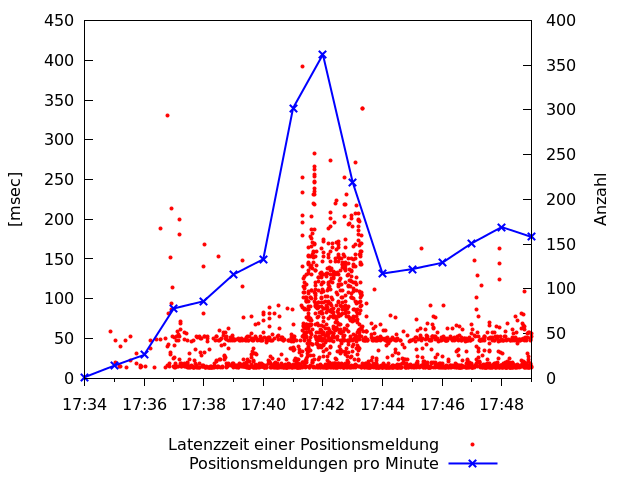
\includegraphics[width=4.5in]{images/latency_timeReceived_socket_io.png}
\end{center}
\caption{socket.io-Websocket-Server: Latenzzeit der Positionsmeldungen und Anzahl empfangener Schiffe}
\end {figure}

\begin {figure}[H]
\begin{center}
  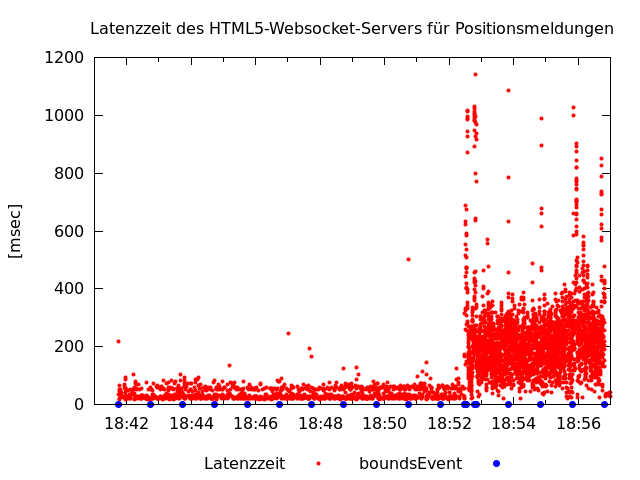
\includegraphics[width=4.5in]{images/latency_timeReceived_HTML5.png}
\end{center}
\caption{HTML5-Websocket-Server: Latenzzeit der Positionsmeldungen und Anzahl empfangener Schiffe}
\end {figure}


\subsection{Performance}
paintToMap

\subsection{Browserunterstützung}
Firefox, Chrome, IE, Safari


\section{Javascript-Client vs. Dart-Client} 
\subsection{Implementierungsaufwand}

\subsubsection{js-Client}
Zeilen Code



\subsection{Latenzzeit}
queryTime

\subsection{Performance}
paintToMap



\begin {figure}[H]
\begin{center}
  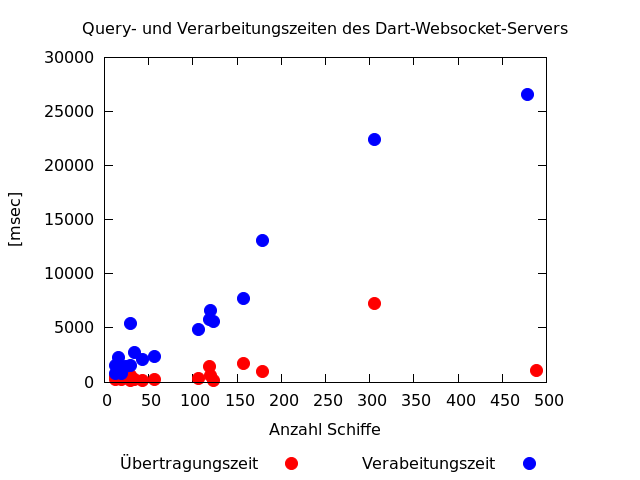
\includegraphics[width=5in]{images/dart.png}
\end{center}
\end {figure}


\subsection{Browserunterstützung}
\subsubsection{Dartium}

\subsubsection{Firefox, Chrome, IE, Safari}

Der dart-Client kompiliert den in Dart geschriebenen Code zu Javascript.

Dabei traten Fehler auf, die unter Dartium (also im originalen Dart-Code) nicht auftraten.
1. Wird innerhalb des Javascript-Scopes eine Methode auf einen javascript-Proxy (hier \_map) aufgerufen und ein proxy wird zurückgegeben, dann ist es nicht möglich auf diesen Proxy, der in diesem Fall vom Typ LatLngBounds sein müsste, eine Methode der Klasse LatLngBounds aufzurufen. => TypeError: t1.get\$\_map(...).getBounds\$0(...).getSouthWest\$0 is not a function

dart-client: web/leaflet\_maps.dart

  List getBounds(){
    var south, west, north, east;
    js.scoped((){
    south= \_map.getBounds().getSouthWest().lng;
        west = \_map.getBounds().getSouthWest().lat;
        north = \_map.getBounds().getNorthEast().lng;
        east = \_map.getBounds().getNorthEast().lat;
 });
return [west, south, east, north];
    
In diesem Fall wird einfach als work-Around eine andere Methode verwendet (getBBoxString), die einen String mit den Bounds zurückgibt. Aus den Teilen dieses Strings werden mit der Methode parse(string) der Klasse double die Werte der Eckpunkte der Bounds generiert.

String getBounds(){
    String bBox;
    js.scoped((){
      bBox = \_map.getBounds().toBBoxString();
    });
    return bBox;
  }

 Weil dadurch der message-Parameter 'bounds' kein number-Array, sondern ein String ist, muss im html5-Server der String einmal zum Float geparst werden.



2. Ein Feld ("IMO") wird auf null und auf > 0 geprüft.


\chapter{Fazit}\label{c.Fazit}

 \section{Ergebnisse }

\section{Ausblick}


\bibliographystyle{alphadin_martin}
%\bibliography{bibliographie}
\begin{thebibliography}{999}
	\bibitem{Ladd12} Seth Ladd, "Sorry, at the time of this writing, I'm not aware of a socket.io port for Dart. socket.io is nice because it has a bunch of implementation options for browsers that don't support Web sockets. Sounds like a good idea for a hackathon project!",2012 Oct 15,  http://stackoverflow.com/questions/12882112/is-there-a-socket-io-port-to-dart.
\end{thebibliography}

%---------------------------------------------------------------------------------------------------------------------------------------------
\chapter*{Erklärung}

Hiermit versichere ich, dass ich die vorliegende Arbeit selbstständig verfasst und keine anderen als die angegebenen Quellen und Hilfsmittel benutzt habe, dass alle Stellen der Arbeit, die wörtlich oder sinngemäß aus anderen Quellen übernommen wurden, als solche kenntlich gemacht und dass die Arbeit in gleicher oder ähnlicher Form noch keiner Prüfungsbehörde vorgelegt wurde.

\vspace{3cm}
Ort, Datum \hspace{5cm} Unterschrift\\

\end{document}